\section{Results}
\label{s:results}

\subsection{RQ1: Requirement-to-License Mapping}
\label{ss:rq1}

\begin{table}[tb]
    \caption{Stage 1 configurations on the same 104 descriptions.}
    \label{tab:stage1}
    \centering
    \footnotesize
    \begin{tabular}{@{}lrrr@{}}
        \toprule
        \textbf{Configuration} & \textbf{Hit@1} & \textbf{Hit@3} & \textbf{Prec@3} \\
        \midrule
        Prompt v1, gpt-oss-120b (Phase 1) & 0.558 & 0.740 & 0.548 \\
        \textbf{Prompt v2, gpt-oss-120b} & \textbf{0.885} & \textbf{0.942} & \textbf{0.849} \\
        Prompt v1, gpt-oss-20b & 0.548 & 0.692 & 0.519 \\
        \bottomrule
    \end{tabular}
\end{table}

\begin{figure}[tb]
    \centering
    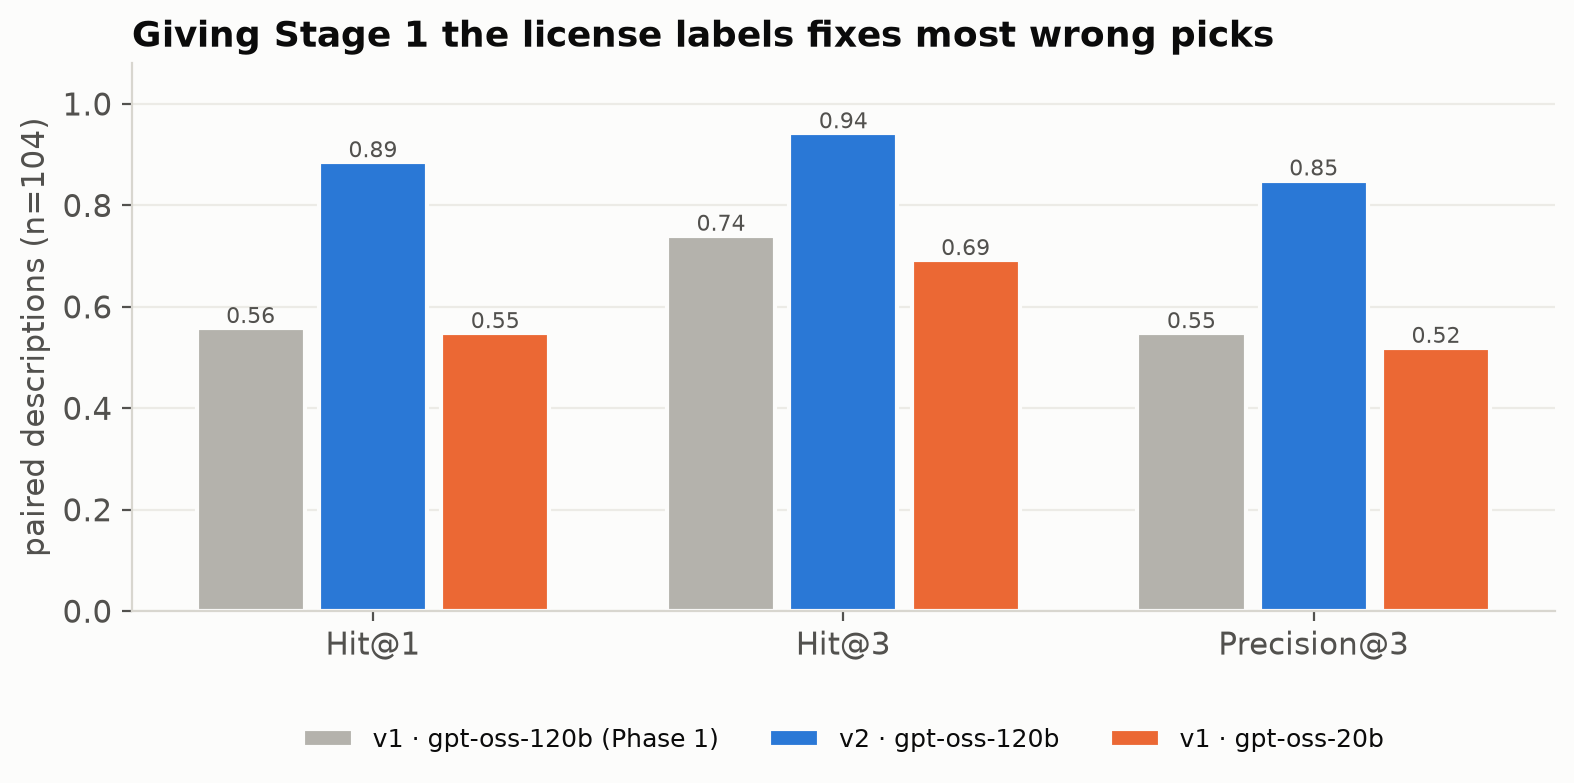
\includegraphics[width=\columnwidth]{p2_05_stage1_configs.png}
    \caption{RQ1: Stage 1 configurations on 104 paired descriptions.}
    \label{fig:stage1}
\end{figure}

Table~\ref{tab:stage1} and Fig.~\ref{fig:stage1} answer the new part of RQ1. Grounding the model in the license labels raised top-pick accuracy from 0.558 to 0.885 and top-3 accuracy from 0.740 to 0.942. The smaller model with the original prompt was slightly worse than the baseline on every metric, so grounding matters far more than model size, and gpt-oss-120b remains the deployed model. The cost is about 40\% more tokens per description, and 6 of 104 requests initially exceeded the free tier's per-minute limit; all succeeded when retried with a smaller output cap.

\begin{table}[tb]
    \caption{Hit@1 / Hit@3 by number of correct licenses (answer-key size).}
    \label{tab:spec}
    \centering
    \footnotesize
    \begin{tabular}{@{}lrcc@{}}
        \toprule
        \textbf{Correct licenses} & \textbf{n} & \textbf{v1 (Phase 1)} & \textbf{v2 (Phase 2)} \\
        \midrule
        1--3 (hardest) & 47 & 0.40 / 0.60 & 0.77 / 0.87 \\
        4--10 & 35 & 0.54 / 0.77 & 0.97 / 1.00 \\
        $>$10 (easiest) & 22 & 0.91 / 1.00 & 1.00 / 1.00 \\
        \bottomrule
    \end{tabular}
\end{table}

Table~\ref{tab:spec} shows the effect of specificity. Prompt v2 is near-perfect when four or more licenses fit, and it nearly doubles top-pick accuracy on the hardest requests (0.40 to 0.77), but those requests remain the weakest group: when only one to three licenses fit, the top three miss every correct license for 13\% of descriptions.

\begin{figure}[tb]
    \centering
    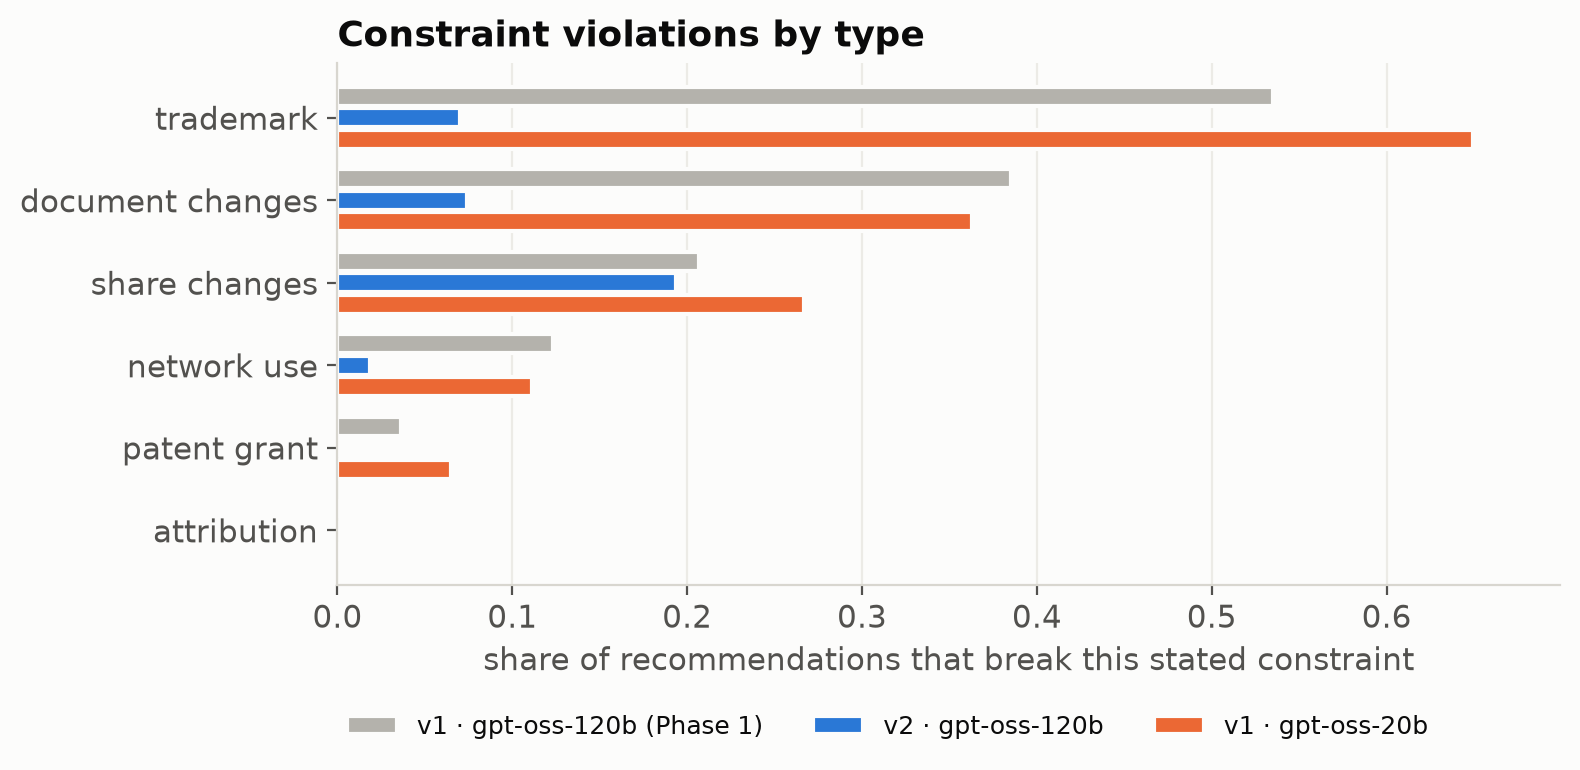
\includegraphics[width=\columnwidth]{p2_06_stage1_violations.png}
    \caption{RQ1: share of recommendations that break each stated requirement.}
    \label{fig:viol}
\end{figure}

Fig.~\ref{fig:viol} shows why. The labels fixed the requirements they state directly: picks that break trademark protection fell from 0.54 to 0.07, change documentation from 0.39 to 0.07, network use from 0.12 to 0.02, and patent grant from 0.04 to 0. The copyleft level barely moved (0.21 to 0.19). Of the 14 descriptions with a copyleft miss, 12 ask for \emph{weak} copyleft (LGPL- or MPL-style, at file or library level), for which only two to four licenses fit; the model mostly falls back to permissive licenses such as Apache-2.0. The v2 prompt explained the trademark, change-documentation, and network labels but not the file- and library-level copyleft labels. We did not patch the prompt after seeing these results, because that would tune it on the test set.

\subsection{RQ2: Claim Verification}
\label{ss:rq2}

\begin{table}[tb]
    \caption{Verifier configurations on 146 human-labelled pairs. Ver.\ prec.\ = verified (entailment) precision; Conf.\ = share of true claims confirmed (entailment recall).}
    \label{tab:verifier}
    \centering
    \footnotesize
    \begin{tabular}{@{}lccc@{}}
        \toprule
        \textbf{Configuration} & \textbf{Acc.} & \textbf{Ver.\ prec.} & \textbf{Conf.} \\
        \midrule
        RoBERTa-large-MNLI (Phase 1) & 0.733 & 0.900 & 0.551 \\
        DeBERTa, argmax (Phase 1) & 0.815 & 0.944 & 0.694 \\
        DeBERTa, threshold $t=0.10$ & 0.829 & 0.925 & 0.755 \\
        Fine-tuned, $K=2$ & 0.897 & 0.936 & 0.898 \\
        \textbf{Fine-tuned, $K=4$} & \textbf{0.925} & \textbf{0.978} & \textbf{0.918} \\
        \midrule
        $K=4$, unseen claim wording & 0.911 & 0.933 & 0.857 \\
        \bottomrule
    \end{tabular}
\end{table}

Table~\ref{tab:verifier} compares the configurations. Threshold tuning alone confirmed 9\% more true claims at a cost of two points of precision. Fine-tuning the top four layers improved every metric: accuracy rose from 0.815 to 0.925 and macro-F1 from 0.816 to 0.925, true claims confirmed rose from 69\% to 92\%, and verified precision rose from 0.944 to 0.978. Training more layers helped ($K=2 \rightarrow 4$) until memory ran out at $K=8$. Because the fine-tuned model's verified precision is already well above the target, it uses the plain argmax rule; the threshold was tuned for the base model.

\begin{figure}[tb]
    \centering
    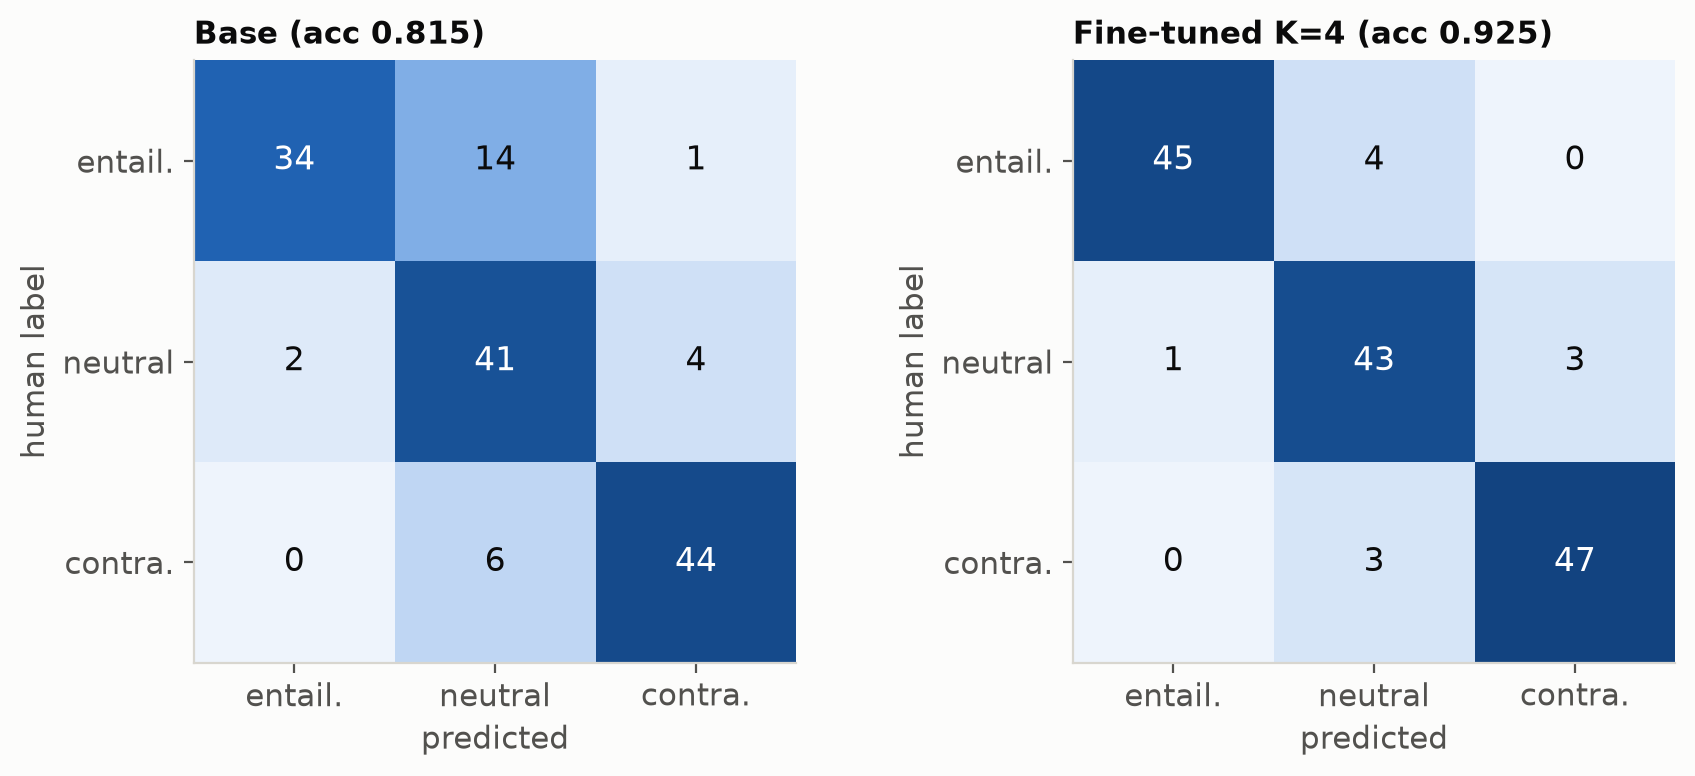
\includegraphics[width=\columnwidth]{p2_03_confusion_base_vs_finetuned.png}
    \caption{RQ2: confusion matrices on 146 human-labelled pairs, base DeBERTa (left) and fine-tuned $K=4$ (right). Rows are human labels.}
    \label{fig:cm}
\end{figure}

Fig.~\ref{fig:cm} shows where the gain comes from. Errors fell from 27 to 11 of 146. True claims judged neutral (shown as \emph{unverified}) fell from 14 to 4. Only one neutral claim was marked verified, and no contradiction was marked verified, so the cautious behaviour that suits licensing is preserved.

\subsubsection{Does the verifier memorise claim wording?}
With folds grouped by label, so that the test claims' wording is never seen in training, accuracy is 0.911, verified precision 0.933, and 86\% of true claims are confirmed (Table~\ref{tab:verifier}, last row). Most of the gain therefore generalises, and the faithfulness target ($\geq 0.90$) is met in both settings. Fig.~\ref{fig:mem} shows the gains per label. Patent-use claims go from 0.41 to 0.94 and trademark claims from 0.55 to 1.00 even with unseen wording. Commercial-use claims, however, rise from 0.21 to 1.00 when the wording was seen but to only 0.33 when it was not: that part of the gain is memorised. With unseen wording, one contradiction was also marked verified (base model: none). We report the unseen-wording score as the honest estimate for new claims.

\begin{figure}[tb]
    \centering
    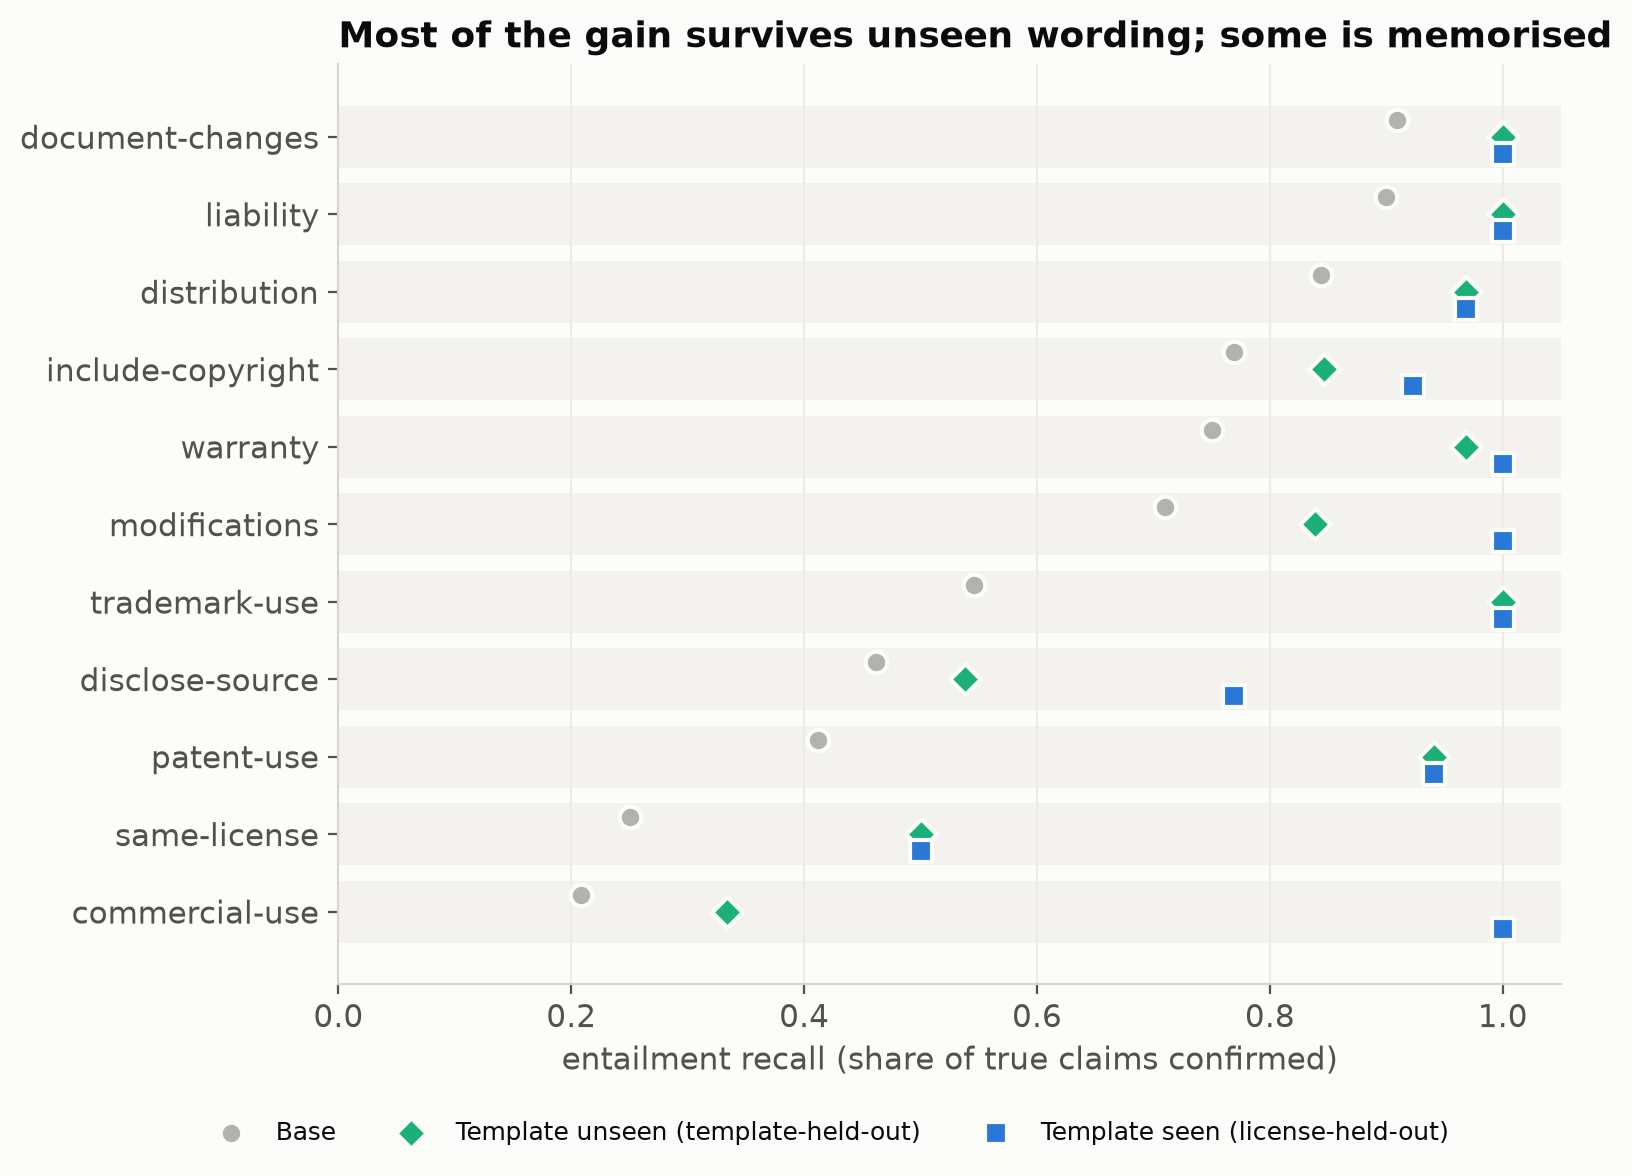
\includegraphics[width=\columnwidth]{p2_04_template_memorisation.png}
    \caption{RQ2: share of true claims confirmed per label for the base model and the fine-tuned model, with claim wording seen and unseen in training.}
    \label{fig:mem}
\end{figure}

\subsection{RQ3: Explanation Faithfulness}
\label{ss:rq3}

In Phase~1, all 19 quotes in two end-to-end runs were found verbatim in their cited clauses, and 58\% of claims were verified. In Phase~2 we re-verified the 37 real Stage~2 claims with a verbatim quote from all saved runs, without new LLM calls, using both verifiers. With the base model, 24 claims were verified, 11 unverified, and 2 contradicted; with the fine-tuned model, 32 were verified, 4 unverified, and 1 contradicted. All eight changed claims read as correct against their clauses, including the Phase~1 false contradiction on AGPL-3.0 section~6. Compared with an unverified (LLM-only) baseline, which would show all 37 claims as equally trustworthy, verification now flags 5 claims for the user to check against the clause instead of 13. This is a preview: these claims are not human-labelled, and the systematic RQ3 study remains future work (Section~\ref{s:future}).

\subsection{Evaluation Against the Requirements}
\label{ss:reqs}

\begin{table}[tb]
    \caption{Phase 2 status against the project requirements.}
    \label{tab:reqs}
    \centering
    \footnotesize
    \begin{tabularx}{\columnwidth}{@{}lX@{}}
        \toprule
        \textbf{Requirement} & \textbf{Phase 2 status} \\
        \midrule
        FR1/FR2 description and/or manifest & Met, in UI and API, validated \\
        FR4 recommend 3 fitting licenses & Met: Hit@3 0.94 (Phase 1: 0.74) \\
        FR5 explain with cited clauses & Met: every claim quotes a clause \\
        FR6 verify each claim & Met: fine-tuned verifier \\
        FR11 operational warnings & Met: rate limit, missing key, invalid input \\
        NFR faithfulness (ver.\ prec.\ $\geq 0.90$) & Met: 0.978; 0.933 on unseen wording \\
        NFR latency ($<$ 5 min, free tier) & Met: about 30--35\,s in our runs; longer when queued or rate-limited \\
        NFR cost & Met: free API tier and a local verifier \\
        NFR security and robustness & Met: type, size, and parse checks before any LLM call; input never executed \\
        NFR reproducibility & Met: pinned dependencies, seeds, tests, CI, decision log \\
        \bottomrule
    \end{tabularx}
\end{table}

Table~\ref{tab:reqs} compares the system with the requirements set in Phase~1. All prioritised functional requirements and the faithfulness requirement are met. Dependency conflicts (FR7) are flagged from declared licenses only; a full compatibility check against the OSADL matrix remains future work.
